\documentclass[a4paper]{ecust_thesis_translation}

\author{赵子川}
\class{计算机095}
\studentNo{10093701}
\title{关于图数据库的调查}
\cKeywords{概念数据库模型,数据库系统,数据模型,图数据模型,图处理语言,图完整性约束}
\eKeywords{Conceptual database models, database systems, database models, graph databases, graph database models, graph query languages, graph integrity constraints}


% 可以按照个人的喜好自行设置字体
% 自行设置字体可参考此处
\setmainfont{Times New Roman}
\setCJKmainfont{SimSun}
\setCJKfamilyfont{hei}{SimHei}
% 请注意:很多中文字体没有粗体的概念,因此在TeX中简单地使用\textbf是
% 不会出现粗体的(摊手),最好使用有独立的粗体和斜体的中文字体。如果使
% 用的字体粗体和斜体是单独的名称,请参考下面格式进行引用。

\begin{document}
% 设置中文缩进
\setlength{\parindent}{2em}
% 设置标点符号挤压模式为半角,可选项有半角、全角、行末半角和开明
\punctstyle{banjiao}

\maketitle

% - 使用\begin{cAbstract} 和 end{cAbstract} 来开始和结束中文摘要
%   模版会自动加载关键词。
\begin{abstract}[chinese]
	图数据库模型可以被定义为概要或实体的数据结构以图或相关结构存储的模型,而数据处理是由面向图论的操作和类型构建而表示的。在八十年代到九十年代初期,这类数据模型与面向对象模型一同蓬勃发展,却在其他数据模型涌现时渐渐隐却,尤其是地理数据库、空间数据库、半结构数据库以及XML数据库。 

	近年来,对于管理现实世界中固有的图状信息的需求使其重新回到相关领域。事实上,随着大规模网络(如互联网,地理系统,运输系统,电话系统)的发展以及由于数据的自发聚集(如生物网络、社交网络)产生的各类网络,一大波全新的、面向图数据库的产品开始出现。 

	本调查的主要目的在于对图数据库建模的进展的研究。着眼于数据结构、查询语句以及完整性约束。
\end{abstract}

\section{导言}
	数据模型这一术语在信息管理组织的定义下有着各种不同的意义和解释。通常来讲,数据模型是一个用来描述一组代表被建模的现实世界实体于实体间的联系的概念性工具的概念[Silberschatz et al 1996]。一般这一术语仅仅表示一组数据结构类型,甚至是用来表示只是的一个数学框架[McGee 1976]。

		\begin{center}
			\begin{figure}[!h]
				\centering
				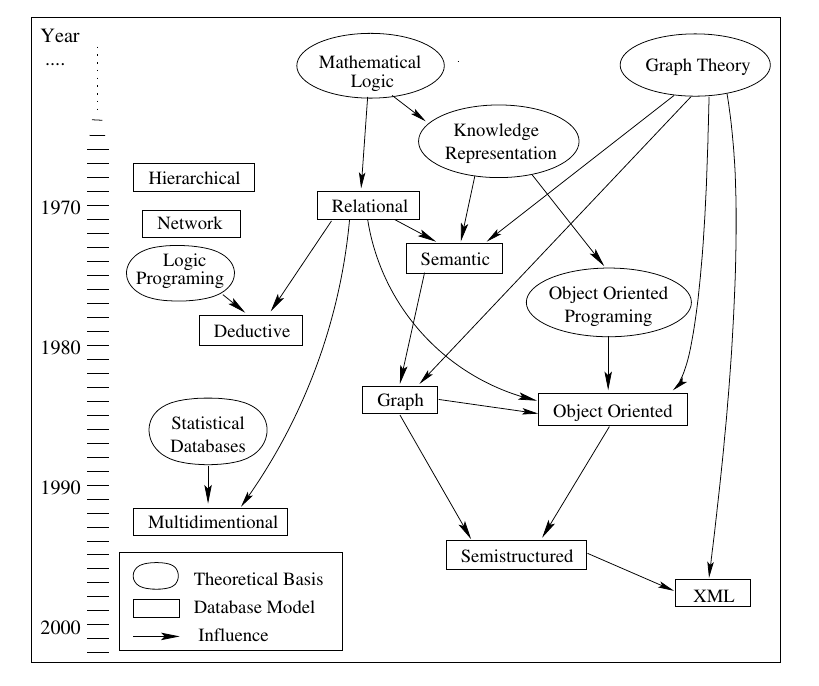
\includegraphics[width=0.95\textwidth]{img/pic1.png}
			\end{figure}
		\end{center}

	从数据库的角度来说,定义数据库模型的概念性工具应当至少指出数据的结构和描述,其可维护性以及获取、查询数据形式。根据这些标准,数据库模型被定义为一个三元组:首先是数据结构类型,其次是一组操作或推理规则,最后是一组普遍完整性规则[Codd 1980]。注意数据库模型的几种方案仅仅定义了数据结构而有时忽略了操作或推理规则。

	由于概念化、哲学化和实用化建模的重要性,数据库模型变成了必要的抽象工具。数据库模型的目的有:制定各类数据的操作权限、数据库的普通设计计量、应对数据库的发展、各类高级数据查询、处理语言的开发、对数据库管理系统架构的关注、结合其他数据组织属性行为的研究成果[Codd 1980]。

	自数据库管理系统诞生以来,关于这类系统所应当使用的数据模型的争论就从未休止。不断进化而趋于多样的现存数据模型表明了在数据建模节是不存在杀手锏的。影响数据库开发的因素是多样的,而最重要的是,建模域的特性与结构、吸引用户的技术性工具、以及由此带来的软/硬件约束都是值得商议的。另外,每一个数据模型方案都基于特定的理论模型,并作为相关模型的发展基础,图1画出了这些影响。

	对数据模型的调查和分类如同数据模型自身一般多样(如. [Silberschatz et al. 1996; Navathe 1992; Beeri 1988; Kerschberg et al. 1976])。

	接下来我们主要介绍最为广泛接受并使用的通用数据模型,也就是,虽然最适合于特定类型的数据,却并不限制某一特定类型的应用。

	\subsection{数据库模型的革命——一个粗略的历史回顾}
		在数据模型设计初期,物理(硬件)限制是纳入考虑的最高因素。在关系模型降临之前,多数数据模型着眼于实际文件系统中的数据。Kerchberg et al. [1976]在1976年前发明了一种分类方法,必要地衡量其数学结构,理论基础和使用的抽象等级。

		两种具有代表性的数据模型是层级模型和网络模型,强调了物理层,并提供了底层操作来实现更加抽象的结构。

		关系数据模型由Codd[1970; 1983]引入,并通过引入区分物理层与逻辑层这一概念提高了抽象等级。它基于集合与关系的概念。由于建模的简易性,其在商业产品中得到了广泛的应用。

		语义数据库模型[Peckham and Maryanski, 1988]使得数据库设计者能够将对象与其关系以一种自然而简洁的方式呈现给用户(相比于之前的模型而言)。他们打算使用工具向用户提供可以表达事物本质的语义信息进行建模。一个著名的例子就是实体关系模型[Chen 1976]。

		面向对象的数据库模型[Kim 1990]出现在80年代,此时大多数的适用新类型的研究关注的是所谓的“为新型产品而设计的先进系统”[Beeri 1988]。这些数据库模型是基于面向对象范型,他们的目标是将数据表示为一组组织为类的,包含复杂数据的对象。

		图数据模型几乎与面向对象数据库同时出现,作为对于传统数据库模型局限性的替代,以捕获应用中的数据固有的图状特性,比如超文本或地理数据库系统,这类数据互联十分重要的领域。

		半结构化数据模型[Buneman 1997]被设计成面向高弹性的数据结构的数据建模模型,比如网页及文档。半结构化数据(又称无结构数据)在常规的数据库中既非严格结构化的,又不能按照原数据存储。另外,该数据模型中数据与架构是浑为一体的,这种特性使得可扩展的数据交换成为可能。这一类数据库模型在90年代出现并踏在数据库革命的征程上。

		XML(eXtensible Markup Language 扩展标记语言)模型[Bray et al.]并非源于数据库。虽然其在一开始作为一种文档交换、建模标准而存在,不久之后其成为了一种通用模型,着眼于树状结构的信息。于半结构化数据相同,这类数据模型是将数据与架构合而为一的。

	\subsection{此次调查的范围,贡献及组织}
		
		本次调查旨在研究对于图数据库及图数据建模领域的进展。在这些调查中,我们更偏向于系统化不同的开发及其相应的要点来引导研究者看清起来元,而非平衡这一领域。这一点非常突出,因为他之前被忽视了,而现在又再一次获得了关注。

		该调查得功能为:

			- 通过提出一个语言上精确而正规的定义将图形数据模型概念化

			- 将图数据模型与其他模型相比较,指出其在特定领域、应用中的特性和问题

			- 定义一组图数据模型的典型特征,比较现有的图数据库模型及基于此标准的研究。我们专注呈现的主要方面是,数据结构,查询语言和完整性约束

			- 提出最适合使用图数据模型的领域

		我们想提醒读者,这个调查的范围下有几个相关的主题。其中最重要的是,我们可以提到图可视化,图数据结构和算法,辅助存储器,图数据库的方法,与一般图形数据库系统的实施。

		在同样的思路下,还有其他一些重要的数据库模型和建模框架涉及图形建模,但由于大小限制,本次调查中,他们这里没有涉及到。如空间数据库模型,地理形成系统(GIS) 时态数据库模型,多维DB-模型。我们的话题集中在数据库在语义网络, 概念图知识表示系统,主题地图,超文本,以及近期发生的家庭表示在Web上的本体模型, OWL上的解决方案。

\section{图数据建模}
	\subsection{什么是图数据模型}
		虽然大多数文件都声称自己使用的是图数据建模的手段,但是对于图数据建模到底是什么并没有一个明确的定义,有的时候这和 数据库 模型没有什么不同。不过对于这种模型,有三个分制,是语义模型,面向对象的模型和半结构话模型。
	
		语义模型是根据模型库,将图转换成语义语言,这种转换有的时候无法保证完整。所以有的时候我们使用图表或者数据结构归纳图。许多研究人员都对对此有一种共识。虽然在大体上这种转化能够符合要求,但是有的时候数据也会有一些细微变化。
		一个图数据库模型是一个被标记的数据有方向性的图。 在这个图中,树枝代表这些模型的连接点。在这个模型中,将这些数据标记,我们就能得到所谓的架构图。一个图数据库也可以表示为一个存储在数据库中的曲线图。这个曲线图是有转换的模型,和对象数据库的实例决定的。曲线图,标记图,组织结构图表可以相互转换。在这些转换图中,标签代表用语架构的关键实例。如果我们将数据库横向处理,我们要考虑架构和实例是否可以被区分,在大部分的情况下,这种担忧是没有必要的。
		
		数据处理是通过图变化得出的结果,他的主要目的是解决典型的特征图,或者向路径,社区,子图,模图,连接或者统计数据。数据库 模式对于收集这些数据的方法很灵活。一般是使用功能强大的源代码。使用者可以通过基于模式的语言,找到实例图。	

		虽然这些方案可以被执行,但是由于架构的不一致会导致身份的不完整,或者功能由于要满足兼容性而大打折扣。所以,标签需要有唯一的名称,在图树的节点上,必须有足够的限制。如果是函数,必须要有定义。对于数据库模型的曲线图汇总,是一种方案。这种模式甚至实例,都会成为面向操作和类型的构造,当有足够的完整性的时候。	对于数据库焦点,需要使用抽象级别的基本数据结构。
	\subsection{为何使用图数据模型}
		图数据库模型的应用范围,这些信息是一样重要的,对于数据本上来说,大部分数据之间都有联系,或者说数据都在相同的水平线只想,事实上,引入图作为建模工具有这样几个有点。	
		\begin{enumerate}
			\item 它导致建模更加自然,对于用户而言,可见的图可以让他们处理运用程序的数据更加自然。图的优点是他可以让数据都显示在一个实体中,并且用信息连接在一起。并且同时可以连接前面的数据和后面的数据。	
			\item 查询数据的时候可以直接引用图的结构,相关的图表可以是的确定分支,或者查询最短路径变的相当容易。书面的程序,或者数据库,都相当复杂,但是一旦使用图库,就会变的很简单。顺便一提,阅览器也是很好用,但是却常常被忘记的架构。	
			\item 如果我们把数据库模型图和数据库草草比较一下的话,我们就会发现模型使得大型的数据集合有了存在的可能性,在最著名的分层或者网络模型中,他们都缺乏良好的抽象水平,并且不灵活。	
		\end{enumerate}
	\subsection{与其他数据模型的比较}
		对于模型来说,从一开始的物理模型,和逻辑电路模型,渐渐的出现了更加形象化的模型,并且使用起来比较简单。(现在的银行,支付,商业还在使用)。	

		这种关系模型是一个里程碑式的发展,由于它提供了一个关于数学的基础模型的规范,基于简单的概念,连同相关的代数和逻辑关系,尤其是它的标准查询转换语言,sql 查询语言,成为了一个典范。	

		在查询语言中,机票预定,会计计算,或者存货分析,都是一向重要的任务,整合模式的不容易,也通常无法自动化,这个时候,我们需要一种没有导向,可以探讨数据之间关系的语言,这种语言可以被用在街区之间的最小路径。	

		面向对象的数据库,鉴于增加了更多的语义集,使得从用户的角度来看,这些东西更加透明,并且可以被轻易使用。这导致了非传统数据库应用程序,例如说 cad/cam 的诞生。	他们都是面向变成对象的很好例子,但是也有不用,ob 主要能够代表一个作为集合的对象。数据库 则能够容纳更加丰富的数据库,但是他们都需要所有的数据符合一个预定义的架构。	

		面向对象的数据库也和这个基本相同,他们提供构建复杂数据相关的对象。对于外表而言,他们是不变的,但是对于接口内部属性,可以根据要求加密。	
		
		即便如此,重要的数据依然在形式之中,面向对象的数据库把系统看成很复杂的对象,而模型图,则强调数据之间的关系,还有他们的属性。	
\section{图数据库模型}
	这一章指出了在图数据库模型中已完成的各类工作。首先,我们提出一个简要的历史回顾的主要建议图数据库模型的形式的区域中的发展情况。然后,我们图数据库模型的主要特点进行了比较研究。

	数据库模型通常通过使用一组共同的特征相比[Fry and Sibley 1976; Tsichritzis and Lochovsky 1976; Peckham and Maryanski 1988]或者定义一个通用的模型作为比较基准[Hull and King 1987]。在本次调查中我们如下评价建模功能,一般考虑三大标准在数据库建模中的概念组织过程:(a)基本模型的基础的数据结构,可在模式和实例级,(b)实现数据一致性(完整性限制)的方法,和(c)查询和操作数据库的语言。 该研究强调概念模型,而不是执行方面的问题。

		\begin{center}
			\begin{figure}[!h]
				\centering
				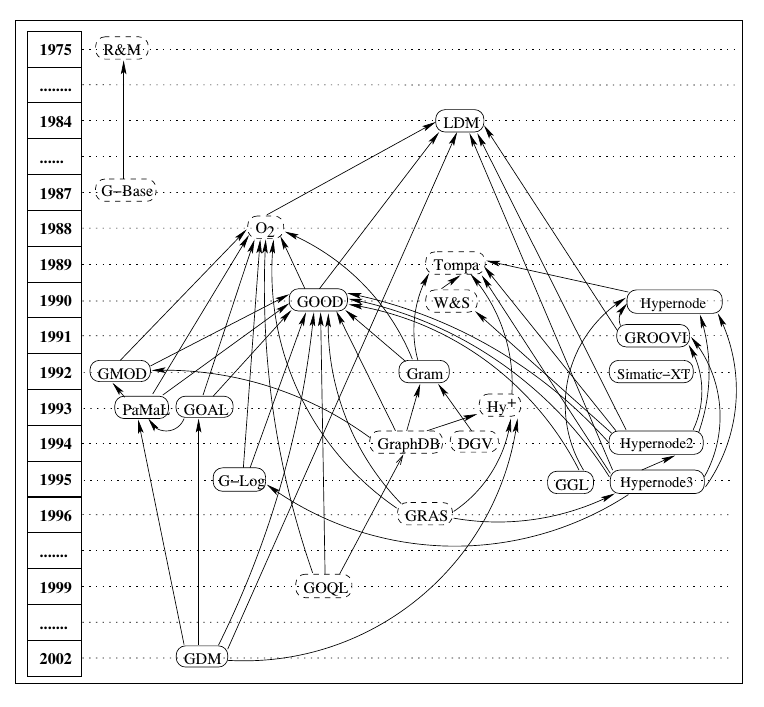
\includegraphics[width=0.95\textwidth]{img/pic2.png}
			\end{figure}
		\end{center}

	\subsection{简略历史回顾}
		围绕图数据库的活动在上半年的20世纪90年代蓬勃发展, 可是接着,这类话题几乎消失了。其原因是多方面的:数据库社区走向半结构化数据(一个研究课题没有链接到图形数据库的工作,在20世纪90年代)的出现、XML捕获所有的注意力工作的人图的超文本的工作、数据库移动到特定的应用程序,如空间数据,网络,文件、对于大多数应用程序类似树的结构是足够的。图2主要通过统计会议和期刊上发表论文的方式反映了这种演变。
			
		图数据库模型的目标模型信息的结构是一个曲线图。在早期的方法中, Roussopoulos和Mylopoulos[1975] 面对当前(在当时)系统的失败,以顾及语义的数据库提出了一种关于数据库的存储数据的语义网络。即一个隐式结构的图形数据本身的功能数据模型[Shipman 1981],其目标是提供一个“在概念上天然的”数据库接口。其他的方法提出了逻辑数据模型(LDM)[Kuper and Valdi1984],作为一个精确的概括来描述关系,层次以及网络模型。数年后Kunii[1987]使用图数据库模型来表示复杂的知识结构,称为G-Base。

		在80年代末, L ́ecluse et al. [1988] 引入了氧气——一个基于图结构的面向对象数据模型。于此同时,GOOD[Gyssens et al, 1990]作为一个有影响力的图形面向对象模型,为透明化图数据操作提供了理论依据。在基于GOOD的各类派生开发中,有提出了面向图形的数据库用户接口概念的GMOD[Andries et al. 1992],用于存储超文本数据的显示图数据库Gram [Amann and Scholl 1992],对GOOD进行了扩充的PaMaL[GEMIS和Paredaens 1993],引入联合节点概念的GOAL[Hidders and Paredaens 1993],提出声明性查询语言的G-Log [Paredaens et al. 1995]以及采用n元对称关系的表示的GDM[Hidders 2002]。

		存在一些概括性图形建模的方案,Levene and Poulovassilis [1990]引入了嵌套的图,成为超点模型。同样的理念被用于为多尺度网络[Mainguenaud 1992]和基因组数据 [Graves et al. 1995]建模。GROOVY[列文 Poulovassilis 1991]是一个使用了超图形式的面向对象数据库模型。在其他情况下使用这种概括:Hy+系统的查询和可视化; 数据实例和模型,对它们的访问,表示用户状态和浏览。

		还有几个处理图数据模型的其他方案,G ̈uting pro- posed GraphDB [G ̈uting 1994] 用于图形对象的建模和查询面向数据库管理信息传输网络中。Database Graph Views [Guti ́errez et al. 1994] 提出了一个抽象的机制来定义和操作存储在关联式的面向对象的图形或文件系统。GRAS项目 [Kiesel et al. 1996] 使用了带键图来为软件工程的复杂信息建模,众所周知的OEM模型 [Papakonstantinou et al. 1995]着眼于提供综合接入异构信息源与信息交流重点。另一项重要的发展,是数据表示模型与万维网。 其中包括像XML [Bray et al. ]的数据交换模型,如RDF[Klyne and Carroll 2004]的元数据表示模型和类似OWL[McGuinness and van Harmelen 2004]的本体表示模型。

\end{document}
